\section{Streaming}
In this section the setup of the two streaming tools GStreamer and CRTMP for \projectname{} will be explained.
Both of these tools will be set up on \deno{S}.
Setting up GStreamer and CRTMP enables that the drone's video stream can be taken as input and displayed in a Flash application.
This is not possible, however, due to the PaVE headers.

\subsection{GStreamer}
\label{sec:GStreamer}
As described in Section~\ref{sec:tools_streaming} the tool GStreamer is used for reading the drone's video stream and forwarding it to CRTMP.
GStreamer is a pipeline based tool that has a command line version which can be run using the \verb+gst-launch-0.10+ command.
The plugins the pipeline consist of are separated by a \verb+!+.
The first plugin in the pipeline is called a source element, and the final element a sink.
The plugins between the source and sink element consist of a set of video and audio processing-, and data management plugins.
A sample pipeline is illustrated in Figure~\ref{fig:sample_pipeline}.

\begin{figure}[htb]
    \centering
    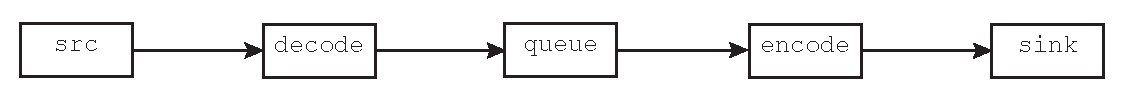
\includegraphics[width=\textwidth]{gfx/sample_pipeline.pdf}
    \caption{Illustration of a sample pipeline.}
    \label{fig:sample_pipeline}
\end{figure}

The source element is capable of receiving a video stream over a specific protocol from a defined source.
As described in Appendix~\ref{app:ar_drone_specification} the drone outputs its video stream using TCP/IP on port 5555, and its IP-address is 192.168.1.1.
To read the stream, the GStreamer plugin \verb+tcpclientsrc+ is used.
The parameters \verb+host+ and \verb+port+ can be set for \verb+tcpclientsrc+.
The first part of the pipeline can be seen in Listing~\ref{lst:tcpclientsrc}.

\begin{lstlisting}[style=sourceCode, language=C, caption=Partial GStreamer pipeline illustrating tcpclientsrc., label=lst:tcpclientsrc]
gst-launch-0.10 tcpclientsrc host=192.168.1.1 port=5555
\end{lstlisting}

The data available to the next plugin is H.264 encoded video with PaVE headers.
The PaVE headers are parsed using the paveparse plugin \citep{paveparse}, as described in Section~\ref{sec:tools_streaming}.
Paveparse removes the PaVE headers and sends the remaining H.264 data down the pipeline.
Furthermore it ignores lost frames and discards frames sent out of order to reduce delay on the stream.
Since the drone streams over TCP/IP and thus no frames are missed, this is necessary to remove potential delay. \\ % and as described in Section~\ref{} \fxfatal{Ref til analysis om hvorfor no delay p� streamen er vigtigt, og check at s�tningen stadig giver mening} delay is not acceptable on the stream. \\

As specified in Section~\ref{sec:technologies} the video output of GStreamer should be in FLV so that the Flash application on \deno{B} can display it.
Two pipelines that output FLV can be created.
The first is using a H.264 decoder to create raw video data, and then encode it as FLV.
The second is using FLVmux.
FLVmux muxes audio and video streams into a single flv file \citep{flvmux}.
However, as the H.264 data has no headers, due to \acs{paveparse}, the H.264 decoder cannot decode the video.
Therefore an FLVmuxer is used to create FLV output. \\

With FLV video outputted from the FLVmuxer, the sink-element can be added to the pipeline.
Since the video stream is forwarded to CRTMP, the sink element is \verb+rtmpsink+.
It has one parameter called \verb+location+, which is the URL-address of the RTMP server with an extension specifying the source-URL of the stream on the RTMP server.
The \verb+rtmpsink+ can be seen in Listing~\ref{lst:rtmpsink}:

\begin{lstlisting}[style=sourceCode, language=C, caption=Partial GStreamer pipeline illustrating rtmpsink., label=lst:rtmpsink]
rtmpsink location='rtmp://0.0.0.0/live/myStream'
\end{lstlisting}

The pipeline that forwards the video stream from the drone can be seen in Listing~\ref{lst:pipeline1}.

\begin{lstlisting}[style=sourceCode, language=C, caption=GStreamer Pipeline with tcpclientsrc and rtmpsink., label=lst:pipeline1]
tcpclientsrc host=192.168.1.1 port=5555 ! paveparse ! flvmux ! rtmpsink location='rtmp://0.0.0.0/live/myStream'
\end{lstlisting}

To handle plugins working at different speeds data management plugins are added to the pipeline.
The plugin used is \verb+queue+.
\verb+queue+ is a data queue that queues data until e.g. the queue reaches a specified size \citep{GStreamer_plugins_queue}.
The \verb+queue+ element is added between every plugin except \verb+tcpclientsrc+ and \verb+paveparse+.  \\

The complete pipeline can be seen in Listing~\ref{lst:pipeline2}:

\begin{lstlisting}[style=sourceCode, language=C, caption=Complete GStreamer Pipeline., label=lst:pipeline2]
tcpclientsrc host=192.168.1.1 port=5555 ! paveparse ! queue ! flvmux ! queue ! rtmpsink location='rtmp://0.0.0.0/live/myStream'
\end{lstlisting}

\subsection{C++ RTMP Server}
\label{sec:CRTMP}
As described in \ref{sec:tools_streaming} \acs{CRTMP} is used as the server tool between GStreamer and the Flash application on \deno{B}.
CRTMP can be executed as a daemon or a console application.
It is configured using a configuration file where its inbound and outbound streams are defined.
The configuration file used in \projectname{} is \verb+flvplayback.lua+, and its relevant content can be seen in Listing~\ref{lst:flvplayback}.
%CRTMP is found at http://www.rtmpd.com and comes in a source package ready to run.
%CRTMP is a standard executable binary. \\
\begin{lstlisting}[style=sourceCode, language=C, caption=Snippet of CRTMP flvplayback.lua Configuration., label=lst:flvplayback]
acceptors =
  {
    {
      ip="0.0.0.0",
      port=1935,
      protocol="inboundRtmp"
    }
  },
externalStreams =
  {
    {
      uri="rtmp://flash.oit.duke.edu/vod/MP4:test/brunswick.m4v",
      localStreamName="test",
      forceTcp=true
    }
  },
\end{lstlisting}


\verb+Acceptors+ define inbound connections to \acs{CRTMP}, meaning which ports users can connect to.
\verb+externalStreams+ define outbound connections to \acs{CRTMP}, meaning the source of the external input.
%\verb+Acceptors+ defines which ports users can connect to and \verb+externalStreams+ define the source of external input.
The \verb+externalSteam+ seen in Listing~\ref{lst:flvplayback} takes a video file from an external server as input, and gives the stream the name \verb+test+.
This test-source was used to test if CRTMP was running correctly.
To view the stream, the program \ac{VLC}, was used, since it has the same capabilities as Flash in regard to streaming RTMP.

A connection is established with a URL-address of the format seen in Listing~\ref{lst:server_address}, where \verb+server address+ is the address of the CRTMP server, \verb+application+ is the application where CRTMP does a lookup e.g. a live-stream or local media, and \verb+streamName+ is the name of the stream.

\begin{lstlisting}[style=sourceCode, language=C, caption=CRTMP URL Format., label=lst:server_address]
rtmp://[server address]/[application]/[streamName]
\end{lstlisting}

When a user connects to CRTMP and the \verb+application+ is live, CRTMP will try to find a live stream that corresponds to the link name.
If no such live stream is found, CRTMP will look in the media folder and try to find file streams.
If no file stream is found, CRTMP will wait for the live stream \verb+streamName+. \\

CRTMP supports user authentication, meaning access to streams can be limited to specific users.
This has however not been implemented in \projectname{}.

%C++ RTMP Server also uses RSA keys.
%It is possible to make users and add these users to realms.
%This can be used as an extra layer of security, but it is not implemented in this version of \projectname{}.

\subsection{Issues with PaVE Headers}
\label{sec:issues_with_pave_headers}
The documentation for the PaVE headers can be found at \citep[page. 59-60]{ardrone_developer_guide}.
As described in Section~\ref{sec:GStreamer}, Flash applications are unable to interpret the PaVE headers.
As a result of this, they are unable to display the video stream.
These headers must therefore be removed or replaced with another header to make the stream readable by Flash.
The implemented solution removes them with the \acs{paveparse} plugin, described in Section~\ref{sec:GStreamer}.
Removing the headers leaves raw video data with no information on how to interpret it.
As a result of this the Flash application and VLC are unable to interpret the video stream.
An illustration of the PaVE header problem can be seen in Figure~\ref{fig:videoframe}. \\

\begin{figure}[htb]
    \centering
    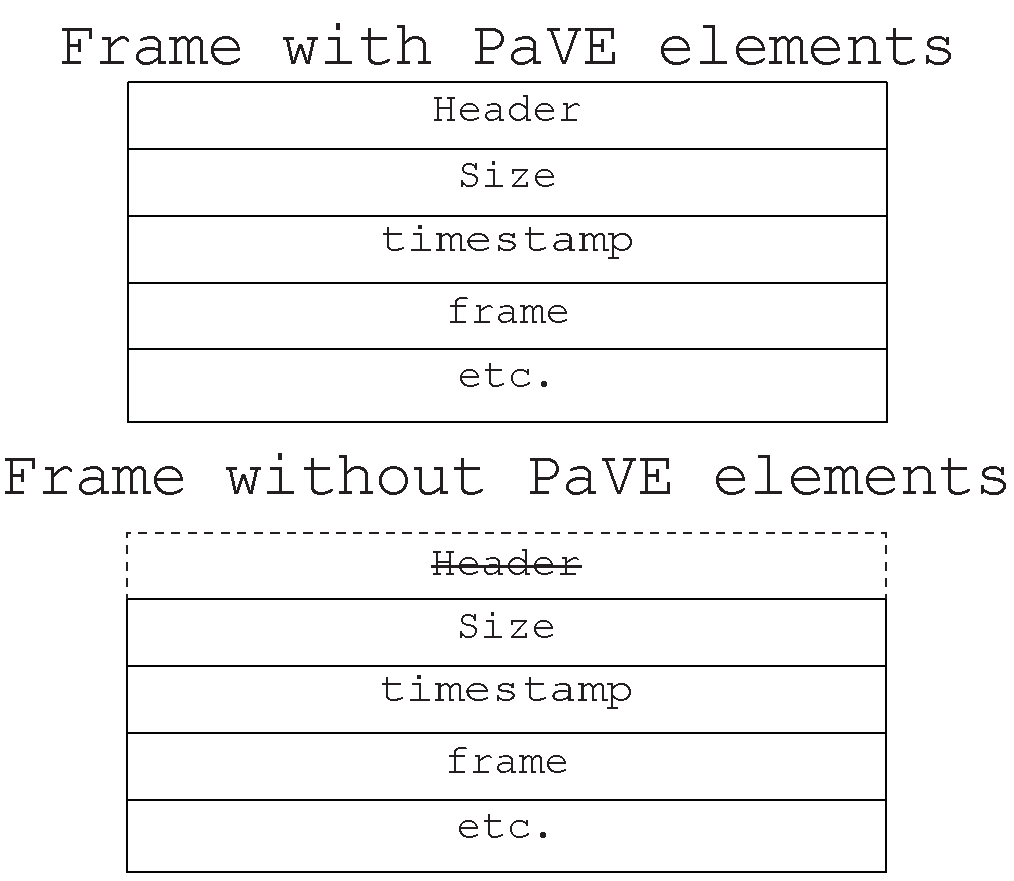
\includegraphics[width=0.7\textwidth]{gfx/videoframe.pdf}
    \caption{Illustration of video frames with and without PaVe headers.}
    \label{fig:videoframe}
\end{figure}

The PaVE headers result in a situation that makes displaying the video stream in Flash impossible, as the video stream cannot be interpreted by a Flash application neither with nor without them.

\subsection{Testing with a Test-input}%\fxfatal{Bedre overskrift}
The designed solution would work if the drone's video stream used standard headers.
The issue is illustrated in Figure~\ref{fig:streaming_issue}.
The goal is to get the stream from the drone, through GStreamer and CRTMP to a Flash application.
The implemented solution is capable of getting the video from the drone to CRTMP, but not capable of generating an output stream readable by Flash.
As illustrated in Case~3 in Figure~\ref{fig:streaming_issue} the setup can forward a stream readable by Flash.
This can be documented by using a different video source as illustrated by Case~4.
For this purpose the GStreamer plugin \verb+videotestsrc+ is used.
It creates a test video stream as seen in Figure~\ref{fig:testvideosrc}, consisting of raw video data.

\begin{figure}[htb]
    \centering 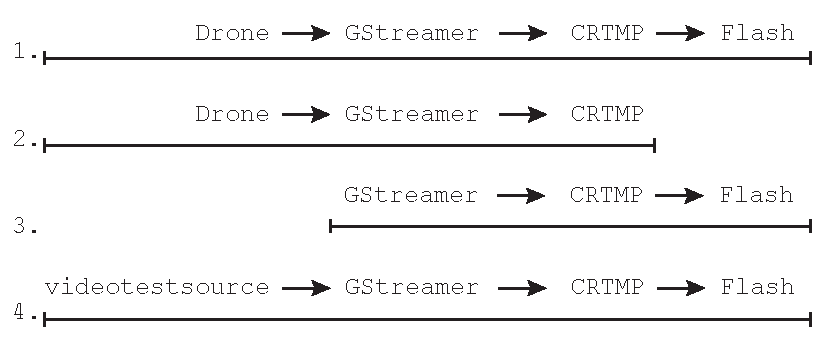
\includegraphics[width=0.8\textwidth]{gfx/streaming_solution.pdf}
    \caption{The Streaming.}
    \label{fig:streaming_issue}
\end{figure}

A \verb+testvideosrc+ pipeline can be seen in Listing~\ref{lst:videotestsrc}.

\begin{lstlisting}[style=sourceCode, language=C, caption=GStreamer Pipeline using videotestsrc., label=lst:videotestsrc]
videotestsrc ! queue ! x264enc ! queue ! flvmux ! queue ! rtmpsink location='rtmp://0.0.0.0/live/myStream'
\end{lstlisting}

If this test-source is used instead of the drone's video stream, it is possible to display the video stream sent by GStreamer. \\

This solution can be seen in Figure~\ref{fig:working_solution}. \\

\begin{figure}[htb]
    \centering
    
\includegraphics[width=0.4\textwidth]{gfx/testvideosrc.pdf}
    \caption{The test video source played with a Flash application.}
    \label{fig:testvideosrc}
\end{figure}

\begin{figure}[htb]
    \centering
    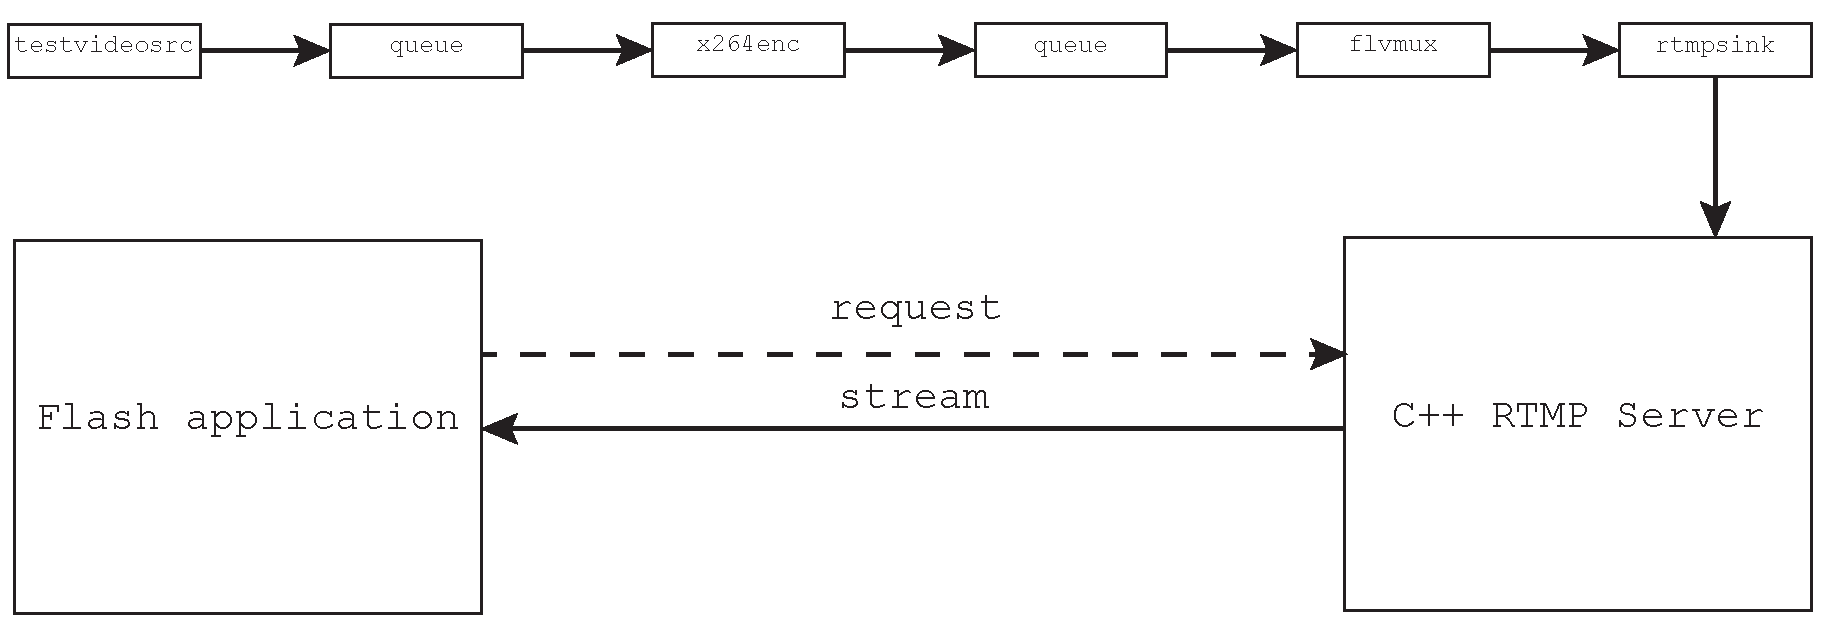
\includegraphics[width=0.8\textwidth]{gfx/Working_solution.pdf}
    \caption{Illustration of the working solution with use of the video test source.}
    \label{fig:working_solution}
\end{figure}

\subsection{Implemented Streaming Solution}%\fxfatal{Bedre overskrift}
\label{sec:video_stream_implemented_solution}

The streaming setup used in \projectname{} uses GStreamer.
One pipeline that reads the drone's video stream and acts as a server, denoted \deno{SP}, and a client pipeline, denoted \deno{CP}, for displaying the video stream on the client side.
The setup can be seen in Figure~\ref{fig:current_solution}.

\begin{figure}[htb]
    \centering
    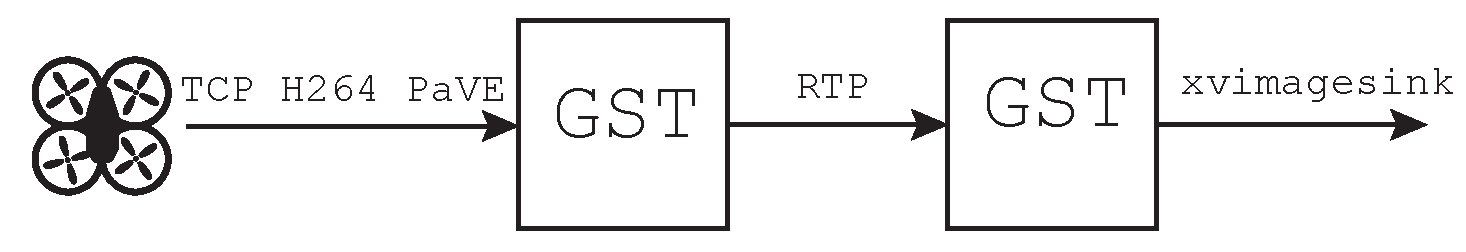
\includegraphics[width=0.7\textwidth]{gfx/current_solution.pdf}
    \caption{Illustration of the implemented solution with xvimagesink.}
    \label{fig:current_solution}
\end{figure}

\deno{SP} reads the drone's video stream and multicasts it using \ac{RTP}.
RTP is a standardized protocol for sending audio and video packages over an IP network.
RTMP is not used, since it is a protocol made specifically for Flash.
RTP is better choice for a solution using only GStreamer, as it is simpler to set up, since it does not have to include settings for the Flash application.
RTP packages are sent via UDP.
\deno{SP} uses the plugins \verb+tcpclientsrc+ and \verb+paveparse+ described in Section~\ref{sec:GStreamer}. \\

Video data sent via RTP must be pay-loaded, since a \acs{Video Frame} is larger than the maximum size allowed size of a UDP packet.
Pay-loading a video stream means encapsulating it into a specific format.
Pay-loading adds the RTP header to the data packages which encapsulates the pay-loaded data.
GStreamer has a set of RTP pay- and depayloaders for each video format it supports.
The plugin used in this pipeline is \verb+rtph264pay+. \\

GStreamer does not have a dedicated RTP sink.
As RTP packages are sent via UDP, the \verb+udpsink+ is used.
\verb+udpsink+ has two parameters, \verb+host+ and \verb+port+, and a set of optional flags with default values.
The flag \verb+auto-multicast+ must be set to true to broadcast the stream globally.
Accordingly the host is set to the multicast IP \verb+224.1.1.1+.
The port is set to \verb+5123+. \\ %as specified in Section\fxfatal{ref til der hvor det kommer}.

The complete \deno{SP} can be seen in Listing~\ref{lst:SP}:

\begin{lstlisting}[style=sourceCode, language=C, caption=rtmpsink setup., label=lst:SP]
tcpclientsrc host=192.168.1.1 port=5555 ! paveparse ! rtph264pay ! udpsink host=224.1.1.1 port=5123 auto-multicast=true
\end{lstlisting}

\deno{CP} uses the \verb+udpsrc+ element to read the video stream.
\verb+udpsrc+ parameters are identical to those of \verb+udpsink+.
In order to decode the stream, an additional parameter named \verb+caps+ must be set.
\verb+caps+ is used to describe metadata about the incoming video stream and contains information such as encoding, the protocol it is being sent using, \acs{Framerate}, etc.
The caps are generated by \deno{SP}.
The \verb+udpsrc+ element of \deno{CP} can be seen in Listing~\ref{lst:udpsrc}. \\

\begin{lstlisting}[style=sourceCode, language=C, caption=udpsrc setup., label=lst:udpsrc]
udpsrc uri=rtp://XXX.XXX.XXX.XXX port=5123 caps = "application/x-rtp, media=(string)video, clock-rate=(int)90000, encoding-name=(string)H264, sprop-parameter-sets=(string)\"Z01AFeygoP2AiAAAAwALuaygAHixbLA\\=\\,aOvssg\\=\\=\", payload=(int)96, ssrc=(uint)1171155755, clock-base=(uint)868988588, seqnum-base=(uint)65233"
\end{lstlisting}
%\fxfatal{Highlighting er m�rkelig i streaming listings}.

The next two steps of the pipeline is depayload the received data and decode it to raw video data.
The depayloading is done with the \verb+rtph264depay+ plugin and the decoding with the \verb+ffdec_h264+ plugin.
Following these two steps, the video data is reassembled and decoded after the transfer.% and then it is being decoded.
The last plugin used is \verb+xvimagesink+ which displays the video stream to the user.
\verb+xvimagesink+ has two flags used to remove delay on the stream named \verb+sync+ and \verb+async+ which are both set to false.
The complete \deno{CP} can be seen in Listing~\ref{lst:CP}. \\

\begin{lstlisting}[style=sourceCode, language=C, caption=Client pipeline., label=lst:CP]
udpsrc uri=rtp://XXX.XXX.XXX.XXX port=5123 caps = "application/x-rtp, media=(string)video, clock-rate=(int)90000, encoding-name=(string)H264, sprop-parameter-sets=(string)\"Z01AFeygoP2AiAAAAwALuaygAHixbLA\\=\\,aOvssg\\=\\=\", payload=(int)96, ssrc=(uint)1171155755, clock-base=(uint)868988588, seqnum-base=(uint)65233" ! rtph264depay ! ffdec_h264 ! xvimagesink sync=false async=false
\end{lstlisting}




%% http://wiki.rtmpd.com/documentation (Maybe this should in bib)